\documentclass[../borwein-lewis_notes.tex]{subfiles}
\begin{document}
\maketitle
\subsection{3.2 The Value Function}
Here is another approach to KKT conditions in the convex case.
Consider the \textit{inequality constrained convex program}
\begin{equation}
\inf\{f(x)\mid g_i(x)\leq 0 \text{ for } i=1,2,\ldots, m,\; x\in \E\},
\label{3.2.1}
\end{equation}
where $f,g_1,g_2,\ldots, g_m:\E\to (-\infty, +\infty]$ are convex 
and satisfy $\emptyset\neq \dom f\subset\cap_i\dom g_i$. Denoting 
the vector with components $g_i(x)$ by $g(x)$, the function $L:\E
\times \R_+^m\to(-\infty, +\infty]$ defined by 
\begin{equation}
L(x;\lambda) = f(x)+\lambda^\top g(x),
\label{3.2.2}
\end{equation}
is called the \textit{Lagrangian}. A \textit{feasible solution} is a 
point $x\in\dom f$ satisfying the constraints. \\
Presently we say a vector $\bar\lambda\in\R_+^m$ is a \textit{Lagrange 
multiplier vector} for a feasible solution $\bar x$ if $\bar x$ 
minimizes the function $L(\cdot;\bar\lambda)$ over $\E$ and 
$\bar \lambda$ satisfies complementary slackness: $\bar\lambda_i=0$ 
if $g_i(\bar x) < 0$.
\begin{proposition}[Lagrangian sufficient conditions (3.2.3)]
\label{3.2.3}
If the point $\bar x$ is feasible for the convex program \eqref{3.2.1}
and there is a Lagrange multiplier vector, then $\bar x$ is optimal.
\end{proposition}
The KKT conditions are a converse to the above when $f,g_i$ are convex.
 We \textit{perturb} the problem \eqref{3.2.1} and 
analyze the resulting \textit{(optimal) value function} $v:\R^m\to[
-\infty, +\infty]$, defined by the equation 
\begin{equation}
v(b) = \inf\{f(x)\mid g(x)\leq b\}.
\label{3.2.4}
\end{equation}
To generalize the definition of convex functions, we introduce the 
\textit{epigraph} of $h$:
\begin{equation}
\epi(h) = \{(y,r)\in\E\times\R\mid h(y)\leq r\},
\label{3.2.5}
\end{equation}
and we say $h$ is a \textit{convex function} if $\epi(h)$ is a convex set.
An exercise shows in this case that the domain 
\begin{equation*}
\dom(h) = \{y\mid h(y)<\infty\}
\end{equation*}
is convex, and that the value function $v$ \eqref{3.2.4} is convex. 
We say $h$ is \textit{proper} if $\dom h$ is nonempty and $h$ never 
takes the value $-\infty$.
\begin{lemma}[3.2.6]
If the function $h:\E\to[-\infty, +\infty]$ is convex and some point 
$\hat y$ in $\core(\dom h)$ satisfies $h(\hat y)>-\infty$, then $h$ 
never takes the value $-\infty$.
\label{3.2.6}
\end{lemma}
Here is a regularity condition called the \textit{Slater constraint 
qualification}, for \eqref{3.2.1}:
\begin{equation}
\text{There exists }\hat x\text{ in }\dom f\text{ with }g_i(\hat x)<0
\text{ for }i=1,\ldots, m.
\label{3.2.7}
\end{equation}
\begin{theorem}[Lagrangian necessary conditions (3.2.8)]
Suppose that the point $\bar x$ in $\dom f$ is optimal for the convex 
program \eqref{3.2.1} and that the Slater condition \eqref{3.2.7} 
holds. Then there is a Lagrange multiplier vector for $\bar x$.
\label{3.2.8}
\end{theorem}
\subsection{Exercises for 3.2}
\textbf{1.} Prove the Lagrangian sufficient conditions \eqref{3.2.3}.
\bluea{
\begin{proof}
Suppose that $\bar x$ is feasible for \eqref{3.2.1} and there is a 
Lagrange multiplier vector $\bar \lambda\in\R_+^m$. Pick any 
feasible $x\in\E$.
\begin{equation*}
f(\bar x) = f(\bar x) + \bar\lambda^\top g(\bar x)
\leq f(x) + \bar\lambda g(x) \leq f(x).
\end{equation*}
The first equality is by complementary slackness ($\bar\lambda^\top 
g(\bar x) = 0$); the first inequality is because $\bar x$ minimizes 
$L(\cdot;\bar\lambda)$ over $\E$, and the last inequality is because 
$x$ is feasible ($g(x)\leq 0).$
\end{proof}
}\noindent
\textbf{2.} Use the Lagrangian sufficient conditions \eqref{3.2.3} to
solve the following problems. 
\begin{enumerate}[(a)]
\item \text{} \vspace{-14pt}
\begin{equation*}
\begin{aligned}
& \inf && x_1^2 + x_2^2 -6x_1-2x_2+10\\
&\text{subject to} &&2x_1+x_2-2\leq 0 \\
&&& x_2-1\leq 0 \\
&&& x\in\R^2.
\end{aligned}
\end{equation*}
\bluea{
The Lagrangian $L(x;\lambda)$ is 
\begin{equation*}
L(x;\lambda) = x_1^2 + x_2^2 - 6x_1-2x_2+10+\lambda_1(2x_1+x_2-2)
+ \lambda_2(x_2-1).
\end{equation*}
For any $\lambda\in\R$, $L(x; \lambda)$ is convex in $x$, being a sum 
of a strictly convex function ($x_1^2 + x_2^2$) and a linear function.
Therefore, by Proposition 2.2 (first order sufficient condition for 
convex functions), the global minimizer in $x$ (for any fixed $\lambda$) 
may be computed by setting the gradient to 0:
\begin{equation}
\begin{bmatrix}
2x_1 - 6 + 2\lambda_1 \\
2x_2 - 2 + \lambda_1 + \lambda_2 
\end{bmatrix}
= \begin{bmatrix}
0\\ 0 \end{bmatrix} 
\iff 
\begin{aligned}
& x_1 = 3-\lambda_1 \\
& x_2 = 1 - \frac{\lambda_1+\lambda_2}{2}
\end{aligned}.
\label{lagrange1}
\end{equation}
The above enables to find a $(\bar x,\bar\lambda)$ satisfying the first
requirement of a Lagrange multiplier vector. We also need to make sure 
$\bar x$ is feasible, and that $(\bar x, \bar\lambda )$ satisfy 
complementary slackness: $\lambda_1(2x_1 + x_2 -2)=0$ and 
$\lambda_2(x_2-1)=0$. If we try setting $x_2=1$, then the second 
equation in \eqref{lagrange1} implies $\lambda_1+\lambda_2=0$, 
which since we need $\lambda\geq0$ implies $\lambda =0$. Then 
\eqref{lagrange1} gives $x_1 = 3$. But then $2x_1 + x_2-2 = 6+1-2 
> 0$, i.e. $x$ is not feasible. \\
Therefore, to satisfy $\lambda_2(x_2-1)=0$, $\lambda_2=0$ necessarily.
 If $\lambda_1=0$, then $x_2 = 1$, which we just ruled out. 
Therefore, $\lambda_1>0$ and to satisfy 
$\lambda_1(2x_1+x_2-2)=0$, $2x_1+x_2-2=0$.
 Plugging in \eqref{lagrange1} with 
$\lambda_2=0$,
\begin{equation*}
6-2\lambda_1 + 1 - \frac{\lambda_1}{2} - 2 
= 5 - \frac{5\lambda_1}{2} = 0 
\implies \lambda_1 = 2.
\end{equation*}
Therefore, our optimal $(\bar x,\bar\lambda)$ pair is 
\begin{equation*}
\bar x =
\begin{bmatrix}
\bar x_1 \\ \bar x_2 
\end{bmatrix} =
 \begin{bmatrix}
1 \\
0 
\end{bmatrix},
\qquad 
\bar\lambda = \begin{bmatrix} \bar\lambda_1 \\ \bar\lambda_2\end{bmatrix}
= \begin{bmatrix}
2 \\ 0
\end{bmatrix}.
\end{equation*}
It can be checked that the optimal objective value is 
$L(\bar x;\bar\lambda) = 5$. Furthermore, $\bar x$ is feasible 
as $2\bar x_1 + \bar x_2 - 2 = 0$ and $\bar x_2 - 1 = -1<0$.
}
\item \text{} \vspace{-14pt}
\begin{equation*}
\begin{aligned}
&\inf &&-2x_1+x_2 \\
&\text{subject to} &&x_1^2-x_2\leq 0\\
&&& x_2-4\leq 0\\
&&&x\in\R^2.
\end{aligned}
\end{equation*}
\bluea{
The Lagrangian for this problem is 
\begin{equation*}
L(x;\lambda)=-2x_1 + x_2 + \lambda_1(x_1^2 - x_2) + \lambda_2(x_2-4).
\end{equation*}
Noting that $L(x;\lambda)$ is convex in $x$ for any $\lambda\geq 0$, 
\begin{equation}
L(x;\lambda) = \inf_{x'\in\R^2} L(x';\lambda) \iff
\begin{bmatrix}
-2 + 2\lambda_1 x_1\\
1 -\lambda_1 + \lambda_2
\end{bmatrix}
= \begin{bmatrix} 0 \\ 0 \end{bmatrix} 
\iff 
\begin{aligned}
&\lambda_1 x_1  = 1 \\
&\lambda_1-\lambda_2 = 1
\end{aligned}.
\label{lagrange2}
\end{equation}
Complementary slackness reads 
\begin{equation}
\lambda_1(x_1^2-x_2) = 0, 
\qquad \lambda_2(x_2-4) = 0.
\label{compslack3.2.2.2}
\end{equation}
Since $\lambda_1x_1=1$, we have $\lambda_1>0$. Then by 
\eqref{compslack3.2.2.2}, $x_1^2 = x_2$. \\
Now suppose $\lambda_2=0$. \eqref{lagrange2} implies $\lambda_1=1 \implies
x_1=1\implies x_2=1$. Thus, 
\begin{equation*}
\bar x = \begin{bmatrix} 1 \\ 1 \end{bmatrix}, 
\qquad \bar\lambda = \begin{bmatrix} 1 \\ 0 \end{bmatrix}
\end{equation*}
satisfy \eqref{lagrange2}, \eqref{compslack3.2.2.2}. $\bar x$ is feasible 
and $\bar\lambda\geq 0$, thus $\bar x$ is optimal. The value is 
$-2\bar x_1 + x_2 = -2$.
}
\item \text{} \vspace{-14pt}
\begin{equation*}
\begin{aligned}
&\inf && x_1+\frac{2}{x_2} \\
&\text{subject to} && -x_2+\frac{1}{2}\leq 0 \\
&&& -x_1+x_2^2 \leq 0 \\
&&& x\in\{(x_1,x_2)\mid x_2>0\}.
\end{aligned}
\end{equation*}
\bluea{
The Lagrangian is 
\begin{equation*}
L(x;\lambda)=
x_1+\frac{2}{x_2} + \lambda_1\left(-x_2+\frac{1}{2}\right)+\lambda_2\left(
-x_1 + x_2^2\right).
\end{equation*}
Notice that the constraint $x_2 \geq \frac{1}{2}$ already implies 
$x\in\{(x_1,x_2)\mid x_2>0\}$. Thus, $L(x;\lambda)$ is convex for 
any feasible $x$ and $\lambda\geq0$. So for feasible $x$,
\begin{equation}
L(x;\lambda)=\inf_{x'\text{ feasible}} L(x';\lambda)\impliedby
\begin{bmatrix}
1-\lambda_2 \\
-\frac{2}{x_2^2} - \lambda_1 + 2\lambda_2x_2
\end{bmatrix}
= \begin{bmatrix} 0 \\ 0\end{bmatrix}
\iff 
\begin{aligned}
&\lambda_2=1\\
& 2x_2^3 - \lambda_1x_2^2 - 2 = 0
\end{aligned}.
\label{lagrange3.2.2.3}
\end{equation}
Complementary slackness is 
\begin{equation}
\lambda_1\left(-x_2+\frac{1}{2}\right)=0,\qquad
 \lambda_2\left(-x_1+x_2^2
\right) = 0.
\label{compslack3.2.2.3}
\end{equation}
Since $\lambda_2=1$ by \eqref{lagrange3.2.2.3}, 
$x_1=x_2^2$ by \eqref{compslack3.2.2.3}.\\
If $\lambda_1=0$, then by \eqref{lagrange3.2.2.3}, 
$2x_2^3-2=0\implies x_2=1$. Then $x_1=x_2^2 = 1$. Thus, 
\begin{equation*}
\bar x = \begin{bmatrix}
1 \\ 1 
\end{bmatrix},
\qquad \bar\lambda  = \begin{bmatrix} 0 \\ 1\end{bmatrix}
\end{equation*}
satisfy \eqref{lagrange3.2.2.3},\eqref{compslack3.2.2.3}. 
Further note that $\bar x$ is feasible and $\bar\lambda\geq 0$. 
Therefore, $\bar x$ is optimal, with value $3$.
}
\end{enumerate}
\textbf{3.} Given strictly positive reals $a_1,a_2,\ldots, a_n, 
c_1,c_2,\ldots, c_n$ and $b$, use the Lagrangian sufficient conditions 
to solve the problem 
\begin{equation*}
\inf\left\{\sum_{i=1}^n \frac{c_i}{x_i}\,\bigg|\,\sum_{i=1}^n a_ix_i
\leq b, x\in\R_{++}^n\right\}.
\end{equation*}
\bluea{
\begin{proof}
The Lagrangian for this problem is 
\begin{equation*}
L(x;\lambda) = \sum_{i=1}^n \frac{c_i}{x_i} + \lambda\left(\sum_{i=1}^n 
a_ix_i - b\right).
\end{equation*}
By convexity of $L(x;\lambda)$ for $x\in\R_{++}^n$, 
\begin{equation}
L(x;\lambda)=\inf_{\text{feasible } x'}L(x';\lambda)\impliedby 
-\frac{c_i}{x_i^2} + \lambda a_i = 0 \iff 
\lambda x_i^2 = \frac{c_i}{a_i} \quad \forall i\in[n].
\label{lagrange3.2.3}
\end{equation}
Complementary slackness says (after using $\lambda > 0$, easy 
from \eqref{lagrange3.2.3})
\begin{equation}
\lambda\left(\sum_{i=1}^n a_ix_i - b\right) =0
\implies \sum_{i=1}^n a_ix_i= b.
\label{compslack3.2.3}
\end{equation}
Utilizing  $\lambda > 0$, we get $x_i = \sqrt{\frac{c_i}{\lambda a_i}}$.
From \eqref{compslack3.2.3}, we get 
\begin{equation*}
\frac{1}{\sqrt{\lambda}}\sum_{i=1}^n \sqrt{a_ic_i} = b 
\implies \sqrt{\lambda} = \frac{\sum_{i=1}^n \sqrt{a_ic_i}}{b}.
\end{equation*}
Thus, $x_i = \frac{b \sqrt{c_i/a_i}}{\sum_{i'=1}^n \sqrt{a_{i'}c_{i'}}}$,
and the optimal objective value is 
\begin{equation*}
\sum_{i=1}^n \frac{c_i}{x_i} = \sqrt{\lambda}\sum_{i=1}^n \sqrt{c_ia_i}
= \frac{\left(\sum_{i=1}^n \sqrt{c_ia_i}\right)^2}{b}.
\end{equation*}
The fact that increasing $a, c$ make the value go up and increasing 
$b$ makes it go down make sense. If $\sqrt{a}$ and $\sqrt{c}$ 
(elementwise) are approximately in the same direction, it becomes 
harder to minimize the objective, and if they are in nearly different 
directions, it becomes easy to minimize the objective.
\end{proof}
}
\noindent
\textbf{4.} For a matrix $A\in\S_{++}^n$ and a real $b>0$, use the 
Lagrangian sufficient conditions to solve the problem 
\begin{equation*}
\inf\{-\log\det X\mid \tr AX \leq b,\, X\in\S_{++}^n\}.
\end{equation*}
You may use the fact that the objective function is convex with derivative 
$-X^{-1}$ (see Section 3.1, Exercise 21 (The log barrier)).
\bluea{
\begin{proof}
The Lagrangian for this problem is 
\begin{equation*}
L(x;\lambda)=-\log\det X + \lambda(\tr AX-b)
\end{equation*}
which is convex in $x$ for $x\in\S_{++}^n$. Thus, 
\begin{equation}
L(x;\lambda)=\inf_{x'\in \S_{++}^n}L(x';\lambda) 
\iff -X^{-1} + \lambda A = 0 
\iff X = \frac{1}{\lambda}A^{-1}.
\label{lagrange3.2.4}
\end{equation}
By complementary slackness, since clearly $\lambda\neq 0$, 
$\tr AX = b$. Thus, right multiplying \eqref{lagrange3.2.4} by $X$ 
and taking the trace, $\tr(-I) + \lambda \tr AX = 0 
\implies \lambda = n/b$. Therefore, $X = \frac{b}{n}A^{-1}$.
This yields objective value 
\begin{align*}
&- \log\det\frac{b}{n} A^{-1}
= -\sum_{i=1}^n \log\lambda(A^{-1})_i - \log(b/n)
= -\sum_{i=1}^n \log\lambda(A)_i^{-1} -\log(b/n)\\
&\quad= \sum_{i=1}^n \log\lambda(A)_i-\log(b/n)
= \log\det A -\log(b)+\log(n).
\end{align*}
\end{proof}
}
\noindent
\textbf{5 * (Mixed constraints).} Consider the convex program 
\eqref{3.2.1} with some additional linear constraints $\ip{a^j, x}=d_j$ 
for vectors $a^j$ in $\E$ and reals $d_j$. By rewriting each equality
as two inequalities (or otherwise), prove a version of the Lagrangian 
sufficient conditions for this problem.
\bluea{
\begin{proof}
Suppose there are $k$ linear constraints $\ip{a^j, x} =d_j$ for 
$j=1,\ldots, k$, which we can express as $h_j(x) = 0$ with 
$h_j(x) = \ip{a^j,x}-d$. We wish to find a version of the Lagrangian 
sufficient conditions for this problem. \\
We begin by casting this problem into the form we already know by 
replacing the constraints $h_j(x) = 0$ with the constraints 
$h_j(x)\leq 0,\, -h_j(x)\leq 0$. As $h$ is affine these constraints 
are all convex, though this does not affect the sufficient condition.
The Lagrangian may be written as $L:\E\times\R_+^m\times \R_+^k\times
\R_+^k\to\R$,
\begin{align*}
L(x;\lambda,\mu^+,\mu^-) &= f(x) + \lambda^\top g(x) + (\mu^+)^\top h(x)
- (\mu^+)^\top h(x)\\
&= f(x) + \lambda^\top g(x) + (\mu^+-\mu^-)^\top h(x).
\end{align*}
The Lagrangian sufficient condition says, if $\bar x$ is feasible, 
$\bar\lambda,\bar\mu^+,\bar\mu^-\geq 0$,
 $\bar x$ minimizes $L(x;\bar\lambda, \bar\mu^+,\bar\mu^-)$ over 
the ``base set'' (e.g. $\R^n$, or $\S_{++}^n$), and complementary 
slackness holds: $\lambda^\top g(\bar x) = 0,\, (\mu^+)^\top h(\bar x) = 0,\, 
(\mu^-)^\top h(\bar x)=0$, then $\bar x$ is an optimal solution to the 
optimization program.\\
Our alternate conditions will be a streamlined way of stating the above.
If $\bar x$ is feasible, then $h(\bar x)=0$ so there is no need for 
the complementary slackness constraints $(\mu^{+,-})^\top h(x) = 0$.\\
Furthermore, notice that any $\mu\in\R^k$ 
can be written as $\mu = \mu^+-\mu^-$ for $\mu^+,\mu^-\in\R_+^k$. \\
Therefore, we can instead look for $(\bar x,\bar\lambda,\bar\mu)$ 
where $\bar\mu\in\R^k$ such that $\bar x$ minimizes 
\begin{equation*}
\cL(x;\bar\lambda,\bar\mu) = f(x) + \bar\lambda^\top g(x) + 
\bar\mu^\top h(x)
\end{equation*}
over the base set. If $\bar x$ is also feasible and $\bar\lambda^\top
g(x)=0$, then the previous sufficient conditions hold (replacing 
$\mu$ with $\mu^+-\mu^-$) and thus $\bar x$ is optimal. \\
Therefore, our new Lagrangian sufficient conditions can be stated as 
finding feasible $\bar x$ and
 $\bar\lambda\in\R_+^m,\, \bar\mu\in\R^k$ such that 
$\cL(x;\bar\lambda,\bar\mu)$ is minimized over $x$ in the base set by 
$\bar x$, and complementary slackness w.r.t the inequality constraints 
holds.
\end{proof}
}
\noindent 
\textbf{6 (Extended convex functions).}
\begin{enumerate}[(a)]
\item Give an example of a convex function that takes the values 
$0$ and $-\infty$. \\
\bluea{
Consider the function $f:\R\to[-\infty,+\infty]$ 
\begin{equation*}
f(x) = \begin{cases} -\infty & x<0\\ 0 &x=0 \\ +\infty & x >0
\end{cases},
\implies \epi(f) = \{(x_1,x_2)\in\R^2 : x_1<0\}
\cup\{(0,x_2)\in\R^2:x_2\geq 0\}.
\end{equation*}
Clearly if $x,y\in\epi f$ with $x_2 < 0$ and $y_2<0$, any convex 
combination of $x$ and $y$ has second coordinate $<0$ and is thus in 
$\epi f$. Now suppose $\lambda\in(0,1)$ and $x,y\in\epi f$ are such 
that $x_2<0$ and $y_2=0$. Then $(\lambda x + (1-\lambda)y)_2 
= \lambda x_2 + (1-\lambda)y_x < 0$, so $\lambda x + (1-\lambda)y
\in \epi f$. \\
If $x,y$ are such that $x_2=y_2=0$, then $x_1\geq 0$ and $y_1\geq 0$,
and thus $\lambda x + (1-\lambda)y$ has second coordinate 0 and first 
coordinate $\geq 0$, making it an element of $\epi f$. \\
This proves that $\epi f$ is convex, i.e. that $f$ is convex.
}
\item Prove the value function $v$ defined by equation \eqref{3.2.4} is 
convex.  \\
\bluea{
Let $\lambda\in[0,1]$ and $(b_1, r_1)$ and $(b_2, r_2)$ be in 
\begin{equation*}
\epi v = \{(b, r)\in\R^{m+1} \mid v(b) \leq r \}
= \{(b,r)\in\R^{m+1} \mid \inf\{f(x)\mid g(x)\leq b\} \leq r\}.
\end{equation*}
Consider the element $z=(\lambda b_1 + (1-\lambda)b_2, \lambda r_1 
+ (1-\lambda)r_2)$. Since $(b_1,r_1)\in \epi v$, there exists 
$x_1\in \E$ with $g(x_1)\leq b_1$ and $f(x_1)\leq r_1$. Similarly,
$(b_2, r_2)\in\epi v$ gives $x_2$ with 
$g(x_2)\leq b_2$ and $f(x_2)\leq r_2$. Applying the original definition 
of convexity,
\begin{gather*}
g(\lambda x_1 + (1-\lambda)x_2) \leq \lambda b_1 + (1-\lambda)b_2 
\quad \text{(component-wise)},\\
f(\lambda x_1 + (1-\lambda)x_2) \leq \lambda f(x_1) + (1-\lambda)
f(x_2) \leq \lambda r_1 + (1-\lambda)r_2.
\end{gather*}
In other words, $\lambda x_1 + (1-\lambda)x_2$ is a certificate 
that $v(\lambda b_1 + (1-\lambda)b_2) \leq \lambda r_1+(1-\lambda)r_2$, 
i.e. $z\in\epi v$. This proves that $v$ is convex.
}
\item Prove that a function $h:\E\to[-\infty, +\infty]$ is convex if 
and only if it satisfies the inequality 
\begin{equation*}
h(\lambda x + (1-\lambda)y) \leq \lambda h(x)+(1-\lambda)h(y)
\end{equation*}
for any points $x$ and $y$ in $\dom h$ (or $\E$ if $h$ is proper) and 
any real $\lambda$ in $(0,1)$. \\
\bluea{
Suppose $f$ is convex and $x,y\in\dom f$. Let $\lambda\in(0,1)$. 
Let $r_1, r_2$ be any values in $\R$ where $f(x)\leq r_1$ and $f(y)
\leq r_2$, in other words $(x,r_1),(y,r_2)\in\epi f$. By convexity, 
their convex combination is in $\epi f$, i.e.
\begin{equation*}
f(\lambda x+(1-\lambda)y) \leq \lambda r_1+(1-\lambda)r_2.
\end{equation*}
WLOG suppose $f(x) = -\infty$. Then, we can take $r_1\to-\infty$ 
to obtain $f(\lambda x+(1-\lambda)y) = -\infty = \lambda f(x) 
+ (1-\lambda)f(y)$. Otherwise, $f(x), f(y)\in\R$, in which case 
we can just take $r_1=f(x)$, $r_2=f(y)$ to get 
$f(\lambda x + (1-\lambda)y) \leq \lambda f(x)+ (1-\lambda)f(y)$. \\
Now suppose that $f$ satisfies the above inequality for 
all points $x,y\in\dom f$. Let $(x_1, r_1)$ and $(x_2,r_2)$ be in 
$\epi f$. Then $x_1,x_2\in\dom f$ (since $f(x_i)\leq r_i<+\infty$), so
\begin{equation*}
\lambda f(x_1 + (1-\lambda)x_2) \leq \lambda f(x_1)
+ (1-\lambda)f(x_2) \leq \lambda r_1 + (1-\lambda)r_2,
\end{equation*}
implying $\epi f$ is convex, i.e. $f$ is convex. \\
If $f$ is proper, then the proof of the second direction does not change
(if the inequality holds for all $x,y\in \E$, clearly it holds for $x,y\in
\dom f$). For the first direction, if $f(x) = +\infty$, then 
$f(\lambda x + (1-\lambda)y) \leq +\infty = \lambda f(x) + (1-\lambda)
f(y)$ since $f(y) > -\infty$ (as $f$ is proper). Therefore, 
the convexity inequality holds for all $x,y\in\E$.
}
\item Prove that if the function $h:\E\to[-\infty, +\infty]$ is 
convex then $\dom h$ is convex.  \\
\bluea{
By the previous part, if $x,y\in \dom h$, then 
\begin{equation*}
h(\lambda x + (1-\lambda)y) \leq \lambda h(x) + (1-\lambda)h(y)
< +\infty
\end{equation*}
for any $\lambda\in[0,1]$, since both $h(x), h(y) < +\infty$. 
Therefore, $\lambda x+ (1-\lambda)y \in \dom h$.
}
\end{enumerate}
\noindent
\textbf{7 (Nonexistence of multiplier).} For the function $f:\R\to
(-\infty, +\infty]$ defined by $f(x) = -\sqrt{x}$ for $x\in\R_+$ and 
$+\infty$ otherwise, show there is no Lagrange multiplier at the optimal 
solution of $\inf\{f(x)\mid x\leq 0\}$.
\bluea{
\begin{proof}
The optimal solution is clearly $x=0$ with value $0$. The 
Lagrangian is $L(x;\lambda)=f(x;\lambda) = f(x) +\lambda x$. 
Given any $\lambda \geq 0$, $0$ cannot be a minimizer of 
$L(\cdot;\lambda)$: if $\lambda = 0$, then any $x>0$ gives 
\begin{equation*}
L(x;\lambda) = -\sqrt{x} < 0 = L(0;\lambda).
\end{equation*}
If $\lambda > 0$, then $x= 1/4\lambda^2$ gives 
\begin{equation*}
L(x;\lambda) = -\frac{1}{2\lambda} + \frac{1}{4\lambda}
= - \frac{1}{4\lambda} < L(0;\lambda).
\end{equation*}
\end{proof}}
\noindent 
\textbf{\green{8}
 (Duffin's duality gap).} Consider the following problem (for 
real $b$): 
\begin{equation}
\inf\{e^{x_2} \mid \|x\|-x_1\leq b,\,x\in\R^2\}.
\label{3.2.9}
\end{equation}
\begin{enumerate}[(a)]
\item Sketch the feasible region for $b>0$ and for $b=0$. \\
\bluea{
For $b=0$, the feasible region is $\{x\in\R^2 | \|x\|\leq x_1\}$, i.e. 
the nonnegative $x$ axis: \\
\begin{tikzpicture}
\draw[->, black] (-2,0) -- (3,0) node[right] {$x$};
\draw[->, black] (0,-1) -- (0,1) node[above] {$y$};
\draw[blue, ultra thick] (0,0) -- (2.93,0);
\end{tikzpicture}\\
For $b>0$, the feasible region is $\{x|\|x\| \leq x_1 + b\}$. 
$\|x\|\leq x_1 + b\iff x_1^2 +x_2^2 \leq x_1^2 + 2x_1 b + b^2
\iff x_2^2 \leq 2x_1 b + b^2$. The first statement is an $\iff$ 
because $x_1+b$ must be nonnegative if it is $\geq \|x\|$. Thus 
for $b=1$, we get the set of $(x,y)\in\R^2$ with $y^2/2 - 1/2 \leq x$, 
or \\
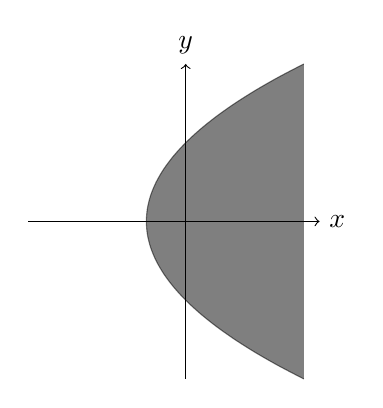
\begin{tikzpicture}
\draw[->, black] (-2,0) -- (1.7,0) node[right] {$x$};
\draw[->, black] (0,-2) -- (0,2) node[above] {$y$};
\draw[domain = -2:2, smooth, variable=\y, fill,
opacity=0.5] plot ({\y*\y*0.5 - 0.5},
{\y});
\end{tikzpicture}
}
\item Plot the value function $v$.  \\
\bluea{
Considering \eqref{3.2.9} as a function $v(b)$ of $b$, the above part 
makes it clear that $v(0) = 1$ (as $x_2=0\implies e^{x_2}=1$) while 
for any $b>0$, $v(b) = 0$ (since the feasible region has a point $x$ 
with $x_2$ arbitrarily small). For $b<0$, $v(b) = +\infty$ as the 
feasible region is empty. 
\begin{tikzpicture}
\draw[black, ->] (-1,0) -- (3,0) node[right] {$x$};
\draw[black, ->] (0, -1) -- (0,2) node[above] {$y$};
\draw[very thick, blue] (0,1)--(0,1.98);
\draw[very thick, blue] (0,0)--(2.98, 0);
\draw[fill=white] (0,0) circle [radius=0.1];
\end{tikzpicture}
}
\item \green{Show that when $b=0$ there is no Lagrange multiplier for any 
feasible solution.} Explain why the Lagrangian necessary conditions 
\eqref{3.2.8} do not apply.  \\
\bluea{
For $x\neq 0$, $\nabla\|x\|=\frac{x}{\|x\|}$ (In Section 3.1, Exercise 
8 we found that $\partial \|x\|=\{x/\\|x\|\}$). Therefore, 
the directional derivative of the Lagrangian in the direction of the 
negative second coordinate is
\begin{equation*}
L'(x;\lambda; -\vec e_2) = 
- L'(x;\lambda;\vec e_2)=-e^{x_2} - \lambda\frac{x_2}{\|x\|}.
\end{equation*}
If $x$ is feasible, $x_2=0$, which means that $L'(x;\lambda;-\vec e_2) = 
-e^{x_2} < 0$. By Proposition 2.1.1 (first order necessary condition), 
$x$ does not minimize $L(\cdot;\lambda)$. \\
If $x=0$, then for $d\in\R^2$,
\begin{align}
\label{ld}
L'(0;\lambda;d) &= \lim_{t\downarrow 0} \frac{e^{td_2} + \lambda(
\|td\|-td_1)- e^0}{t} = d_2 + \lambda(\|d\|-d_1).
\end{align}
If $\lambda=0$ then we can take $d_2 < 0$ to make $L'(0;\lambda;d)<0$.
If $\lambda>0$, then for $d_1>0$,
\begin{align*}
L'(0;\lambda;d) &= d_2+\lambda(\sqrt{d_1^2+d_2^2}-d_1)
= d_2 + \lambda(d_1\sqrt{1+\frac{d_2^2}{d_1^2}} - d_1)\\
&\leq d_2 + \lambda(d_1(1+\frac{d_2^2}{2d_1^2})-d_1)
= d_2 + \lambda\frac{d_2^2}{2d_1}.
\end{align*}
We can take $d_1=1$ and $d_2 = -\frac{1}{2\lambda}$ to et 
$L'(0;\lambda;d) = -\frac{1}{4\lambda} < 0$. This proves that 
$0$ does not minimize $L(\cdot;\lambda)$ either. Thus, there is no 
Lagrange multiplier. \\
Theorem 3.2.8 \eqref{3.2.8} does not apply because the Slater condition
does not hold when $b=0$: $|x|-x_1\leq 0$ must always be satisfied 
with equality.
}
\item Repeat the above exercises with the objective function $e^{x_2}$ 
replaced by $x_2$.\\
\bluea{
The feasible region stays the same so there is no need to repeat 
part (a). To calculate the value function, note that for $b<0$ 
still $v(b) = +\infty$ as the feasible set is empty and 
$v(0) = 0$ since $x_2=0$. For $b>0$, since $x_2$ can get arbitrarily 
small $v(b) = -\infty$. One might plot $v$ as \\
\begin{tikzpicture}
\draw[black, ->] (-1,0) -- (2,0) node[right] {$x$};
\draw[black, ->] (0, -1.5) -- (0,1.5) node[above] {$y$};
\draw[blue] (-0.05,0)--(-0.05,1.48);
\draw[blue] (0.05, 0)--(0.05, -1.48);
\draw[fill=blue] (0,0) circle [radius=0.07];
\end{tikzpicture}
\\
The Lagrangian when $b=0$ is 
\begin{equation*}
L(x;\lambda) = x_2+\lambda(\|x\|-x_1).
\end{equation*}
For any feasible $x$, $L(x;\lambda)=0$. In fact, $L(d;\lambda)$ is 
equal to \eqref{ld} from part (c), for which we showed there is a 
$d\in\R^2$ returning a negative value. In this case, it means 
there is a (non-feasible) $x\in\R^2$ such that $L(x;\lambda) < 0 
= L(x';\lambda)$ for any feasible $x'$, meaning $\lambda$ cannot 
be a Lagrange multiplier.
}
\end{enumerate}
\noindent
\textbf{9 ** (Karush-Kuhn-Tucker vectors [167]).} Consider the convex 
program \eqref{3.2.1}. Suppose the value function $v$ given by 
equation \eqref{3.2.4} is finite at 0. We say the vector $\bar\lambda 
\in\R_+^m$ is a \textit{Karush-Kuhn-Tucker vector} if it satisfies 
$v(0) = \inf\{L(x;\bar\lambda)\mid x\in\E\}$.
\begin{enumerate}[(a)]
\item Prove that the set of Karush-Kuhn-Tucker vectors is $-\partial 
v(0).$ \\
\bluea{
Let $\bar\lambda\in\R_+^m$ be a KKT vector and $b\in\R^m$. Then, 
\begin{align*}
v(0) &= \inf\{f(x) + \bar\lambda^\top g(x) : x\in \E\}
\leq \inf\{f(x) + \bar\lambda^\top g(x) : g(x) \leq b\} \\
&\leq \inf\{f(x) : g(x)\leq b\} + \bar\lambda^\top b 
= v(b) + \bar\lambda^\top b.
\end{align*}
The second inequality follows because when $g(x)\leq b,$ it follows 
that $\bar\lambda^\top g(x)\leq \bar\lambda^\top b$ as $\bar\lambda\geq0$.
Rearranging, we obtain that $-\bar\lambda\in\partial v(0)$. \\
Now if $-\lambda\in\partial v(0)$, since $v(b)\leq v(0)$ for any 
$b\geq0$ we obtain $v(0) \leq v(b)+\bar\lambda^\top b \leq v(0) + 
\bar\lambda^\top b$. This implies that $\bar\lambda\geq 0$. By 
definition of $v$, $f(x)\geq v(g(x))$. Thus, 
\begin{equation*}
f(x)\geq v(g(x)) \geq v(0)-\bar\lambda^\top g(x).
\end{equation*}
I.e., $v(0) \leq f(x)+\bar\lambda^\top g(x)$ for every $x\in \E$.
Thus, $v(0) \leq \inf\{L(x;\bar\lambda)\}$.
On the other hand, since any $\bar x$ with $g(\bar x) \leq 0$ 
satisfies $f(\bar x) + \bar\lambda^\top g(\bar x) \leq f(\bar x)$, 
we have $\inf\{L(x;\bar\lambda)\} \leq v(0)$. This proves that 
$v(0) = \inf\{L(x;\bar\lambda)\}$ and that $\bar\lambda$ is a KKT
 vector.
}
\item Suppose the point $\bar x$ is an optimal solution of problem 
\eqref{3.2.1}. Prove that the set of Karush-Kuhn-Tucker vectors 
coincides with the set of Lagrange multiplier vectors for $\bar x$.\\
\bluea{
Let $\bar\lambda\in\R_+^m$ be a Lagrange multiplier vector. Then, 
\begin{align*}
v(0) = f(\bar x) = f(\bar x)+\bar\lambda^\top g(x) 
= \inf\{L(x;\bar\lambda):x\in\E\}.
\end{align*}
Therefore, $\bar\lambda$ is a KKT vector. \\
Now suppose $\bar\lambda\in\R_+^m$ is a KKT vector. Then 
\begin{equation*}
f(\bar x) +\bar\lambda^\top g(\bar x) \geq \inf\{f(x)+\bar\lambda^\top 
g(x)\} = v(0) = f(\bar x) \geq f(\bar x)+\bar\lambda^\top g(\bar x).
\end{equation*}
The first equality is since $\bar\lambda$ is a KKT vector, and the 
last inequality is because $g(\bar x)\leq 0$ while $\bar\lambda\geq0$.
This proves both that $\bar\lambda^\top g(\bar x) = 0$, i.e. 
complementary slackness, and that $f(\bar x)+\bar\lambda^\top g(\bar x)
= \inf\{L(x;\bar\lambda):x\in\E\}$, i.e. $\bar\lambda$ is a Lagrange 
multiplier vector.
}
\item Prove the Slater condition ensures the existence of a 
Karush-Kuhn-Tucker vector.  \\
\bluea{
The Slater condition ensures that $0\in\core(\dom v)$. By Lemma 
3.2.6 \eqref{3.2.6}, $v$ never takes the value $-\infty$. Then, 
by Theorem 3.1.8, $\partial v(0)$ is nonempty. I.e., by part (a), 
there exists a KKT vector. (\green{proof uses convexity of 
\eqref{3.2.1}}).
}
\item Suppose $\bar\lambda$ is a Karush-Kuhn-Tucker vector. Prove a 
feasible point $\bar x$ is optimal for problem \eqref{3.2.1} if 
and only if $\bar\lambda$ is a Lagrange multiplier vector for $\bar x$.
\\
\bluea{
If $\bar x$ is optimal, then by part (b), $\bar\lambda$ is a Lagrange 
multiplier vector for $\bar x$. \\
If $\bar\lambda$ is a Lagrange multiplier vector for $\bar x$, 
then by Proposition 3.2.3 \eqref{3.2.3}, $\bar x$ is optimal.
}
\end{enumerate}
\noindent
\textbf{10. }Prove the equivalence of the Slater and Mangasarian-Fromovitz
conditions asserted at the end of the section. 
\bluea{
\begin{proof}
Suppose $g_1,\ldots, g_m$ are differentiable. \\
Suppose the Slater condition holds, that is there exists 
$\hat x\in \dom f$
such that $g(\hat x)<0$. Now let feasible $x\in \E$ and let $I(x)$ be the 
set of tight constraints for $x$, $I(x)=\{i\in[m]:g_i(x)=0\}$. For 
each $i\in I,\, g_i(x+t(\hat x-x))$ is convex. Thus, $g_i(x+t(\hat x-x))/t$
is increasing in $t$, and
\begin{equation*}
\ip{\nabla g_i(x), \hat x-x} = \lim_{t\downarrow 0}\frac{g_i(x+t(\hat x
- x)-g(x)}{t} \leq g_i(\hat x) - g_i(x) = g_i(\hat x) < 0.
\end{equation*}
Therefore, $\hat x - x$ is a certificate for the Mangasarian-Fromovitz 
condition. \\
Now suppose that the Mangasarian-Fromovitz condition holds, i.e. 
there exists $d\in\E$ such that $\ip{\nabla g_i(x), d} < 0$ for all 
$i\in I(x)$. Then for all $t>0$ small enough, $g_i(x+td) < g_i(x)=0$ 
for every $i\in I(x)$. If we pick $t>0$ even smaller enough, 
then for every $i\notin I(x)$ we still have $g_i(x+td)<0$ by 
continuity of $g$ (which follows from differentiability).
\end{proof}}
\noindent
\textbf{11 (Normals to epigraphs).} For a function $f:\E\to(-\infty, 
+\infty]$ and a point $\bar x$ in $\core(\dom f)$, calculate the 
normal cone $N_{\epi f}(\bar x, f(\bar x))$. 
\bluea{
\begin{proof}
\begin{equation*}
N_{\epi f}(\bar x, f(\bar x))
 = \{(d,c)\in\E\times \R: \forall (x,r)\in\epi f, \; 
d^\top (x-\bar x)+c(r-f(\bar x)) \leq 0\}.
\end{equation*}
The condition can be written as 
\begin{equation*}
\forall x\in\dom f,\, r\geq f(x),\,
 \ip{d, x-\bar x} \leq -c(r-f(\bar x)),
\end{equation*}
since $(x,r)\in\epi f\implies x \in\dom f$. If $c<0$, then 
the above holds iff $-d/c$ is a subgradient. If $c=0$, then since 
$\bar x\in\core(\dom f)$, we need $d=0$. If $c>0$, then 
for any $x\in\E$, we can take $r\to+\infty$ to reach a contradiction.
Thus, $N_{\epi f}(\bar x, f(\bar x))=\{(-c\phi, c)\in\E\times\R_-:
\phi\in\partial f(\bar x)\}$.
\end{proof}}
\noindent
\textbf{\red{12 (Normals to level sets).}} Suppose the function $f:\E\to
(-\infty, +\infty]$ is convex. If the point $\bar x$ lies in 
$\core(\dom f)$ and is not a minimizer for $f$, prove that the normal 
cone at $\bar x$ to the level set 
\begin{equation*}
C=\{x\in\E\mid f(x)\leq f(\bar x)\}
\end{equation*}
is given by $N_C(\bar x)=\R_+\partial f(\bar x)$. Is the assumption 
$\bar x\in\core(\dom f)$ and $f(\bar x)>\inf f$ necessary? 
\bluea{
\begin{proof}
Suppose that $\phi\in\partial f(\bar x)$. Then, for any $x\in C$, 
$\ip{\phi, x-\bar x}\leq f(x)-f(\bar x) \leq 0$, i.e. $\phi\in 
N_C(\bar x)$. Since $N_C(\bar x)$ is a cone, this implies 
$\R_+\partial f(\bar x)\subset N_C(\bar x)$. \\
Now suppose that $d\in N_C(\bar x)$. We begin by noting that 
\begin{equation}
\label{normineq}
f'(\bar x; d') < 0 \implies \ip{d, d'} < 0.
\end{equation}
 To the contrary, suppose
that $f'(\bar x; d')  < 0$ while $\ip{d, d'} = 0$. Consider for some 
small $s>0$ the directional derivative in the direction 
$d'+sd$. By sublinearity of the directional derivative at 
$\bar x\in\core(\dom f)$ (Proposition 3.1.2),
\begin{equation*}
f'(\bar x; d' + sd) \leq f'(\bar x; d')+sf'(\bar x; d) < 0
\end{equation*}
if we pick $s$ small enough. This implies for some $t>0$ that 
\begin{equation*}
f(\bar x + t(d'+sd)) - f(\bar x) < 0
\end{equation*}
yet $\ip{d, t(d'+sd)} = ts\ip{d,d} > 0$, which contradicts the fact 
that $d\in N_C(\bar x)$. \\
Furthermore, we'll show 
\begin{equation}
\label{normeq}
f'(\bar x; d')= 0 \implies \ip{d, d'} \leq 0.
\end{equation}
Since $\bar x$ is not a minimizer, there is 
a point $x\neq\bar x$ with $f(x)< f(\bar x)$, 
so that if $d'' := x-\bar x$ then $\ip{d, d''} < 0$. By sublinearity, 
we have $f'(\bar x; d' + td'') \leq f'(\bar x; d') + tf'(\bar x; d'')
 < 0$ for any $t>0$ since $f'(\bar x; d')=0$ and $f'(\bar x, d'') < 0$.
 Thus, by \eqref{normineq}, $\ip{d, d'+td''} < 0$,
which since $t>0$ is arbitrary implies $\ip{d, d'}\leq 0$. 
\\
We'll proceed by showing two properties of any sublinear $g$ in relation
to a linear function $\ip{d,\cdot}.$\\
First we'll show that if \eqref{normineq} and \eqref{normeq} hold with 
$g(d')$ in place of $f'(\bar x;d')$, and $g$ is finite everywhere,
 then there exists a $C>0$ such 
that $g(d_1) \geq C\ip{d,d_1}$ for any $d_1$ where $g(d_1)\leq 0$.
Consider the set $D_1 := \{d_1\in\E: g(d_1)=-1\}$. By \eqref{normineq},
for all $d_1\in D_1,\, \ip{d,d_1} < 0$. Therefore, the set 
\begin{equation*}
S := \{-\ip{d,d_1}\mid d_1\in D_1\}
\end{equation*}
is a set of positive reals. Suppose elements of $S$ get arbitrarily
close to 0, i.e. 
there exists a sequence $(d_1^i)_{i=1}^\infty$ such that $-\ip{d,
d_1^i}\downarrow 0$. Then $\ip{d, \frac{d_1^i}{\ip{d,d_1^i}}} = 1$ 
while $g(-\frac{d_1^i}{\ip{d,d_1^i}}) = -\frac{1}{\ip{d,d_1^i}}g(d_1^i)
= \frac{1}{\ip{d,d_1^i}} \to -\infty$.
 Consider the set $H:=\{\hat d_1\in \E: 
\ip{d,\hat d_1} = -1\}$. The sequence $(-\frac{d_1^i}{\ip{d, d_1^i}})_{
i=1}^\infty$ is contained in $H$. Take some $d_0\in H$. By Section 
1.1 Exercise 12, $H-d_0$ is a linear subspace containing 
$(s_i)_{i=1}^\infty
=(-\frac{d_1^i}{\ip{d,d_1^i}}-d_0)_{i=1}^\infty.$ \\
For any $M>0$, there exists $N$ such that $i>N$ implies 
$g(s_i+d_0) \leq -M$. Since $g(s_i+d_0)\geq g(s_i)-g(-d_0)$, 
we have $g(s_i) \leq -M+g(-d_0)$. \\
 Then, $g(-s_i-d_0) \geq g(-d_0) - g(s_i) \geq M$, and 
$g(s_i-d_0)\leq g(s_i) + g(-d_0)\leq -M + 2g(d_0)$. 
If $M$ is
large enough, then $g(-s_i-d_0)>0$ while $g(s_i-d_0) < 0$. Thus, by
continuity of $g(\cdot s_i - d_0)$ 
(HEHEHE unproved XD) there exists a $t\in\R$ such that 
$g(ts_i - d_0) = 0$. On the other hand, $\ip{d, ts_i-d_0} 
= -\ip{d, -ts_i+d_0} = 1$, since $ts_i\in H-d_0 \implies 
-ts_i\in H-d_0$ by linearity. But, $g(ts_i-d_0)=0$ while 
$\ip{d, ts_i-d_0}=1$ contradicts \eqref{normeq}. Therefore, 
$\inf S = C > 0$. Thus, for any $d_1\in D_1, g(d_1) = -1 \geq 
\ip{\frac{d}{C}, d_1}$. Then for any $d_1$ where $g(d_1)<0$, 
we have $g(d_1) \geq \ip{\frac{d}{C},d_1}$, by scaling. If 
$g(d_1)=0$ by \eqref{normeq} $\ip{d,d_1}\leq 0$. Furthermore,
there exists a sequence $d_1^i$ such 
that $g(d_1^i) = -1$ while $\ip{\frac{d}{C}, d_1^i}\uparrow -1$.
\\
Now we will show for any sublinear $g$, if 
$\ip{d, d_1} \leq g(d_1)$ for any 
$d_1\in\{d_1\in \E: g(d_1) \leq 0\}$ and there exists a sequence 
$d_1^i$ such that $g(d_1^i)=-1$ while $\ip{d, d_1^i}\uparrow -1$,
then $g(\cdot)\geq \ip{d,\cdot}$.
For any $d_2\in \E$ such that $g(d_2)>0$,
\begin{align*}
&g(d_2+g(d_2)d_1^i) \leq g(d_2) + g(d_2)g(d_1^i) 
= g(d_2) -g(d_2)= 0, \\
&\implies g(d_2) \geq
g(d_2+g(d_2)d_1^i) - g(d_2)g(d_1^i) \\
&\qquad\geq \ip{d, d_2+g(d_2)d_1^i} - g(d_2)(\ip{d, d_1^i}+\epsilon)\\
&\qquad = \ip{d,d_2}
- g(d_2)\epsilon.
\end{align*}
By taking $i\to\infty$ we can let $\epsilon>0$ be arbitrary, i.e. 
$g(d_2) \geq \ip{d,d_2}$. Since $g(d_1)\geq \ip{d,d_1}$ already 
for all $d_1$ with $g(d_1)\leq 0$, we have $g(\cdot)\geq \ip{d,\cdot}$. \\
Since we proved $f'(\bar x; \cdot)$ satisfies \eqref{normineq} and 
\eqref{normeq} and is finite, with $g=f'(\bar x;\cdot)$ we have
 $g(d_1)\geq C\ip{d, d_1}$ for all 
$d_1$ with $g(d_1)\leq 0$, and a sequence $d_1^i$ such that 
$g(d_1^i)=-1$ while $\ip{Cd,d_1}\uparrow -1$. Then, we have by the 
next result $g(\cdot)\geq \ip{Cd, \cdot}$, which implies that 
$Cd\in\partial f(\bar x)$. Therefore, $N_C(\bar x)\subset \R_+\partial 
f(\bar x)$.
\end{proof}
}
\noindent 
\textbf{13 * (Subdifferential of max-function).} Consider 
convex functions 
\begin{equation*}
g_1,g_2,\ldots, g_m:\E\to(-\infty, +\infty],
\end{equation*}
and define a function $g(x)=\max_i g_i(x)$ for all points $x\in\E$. For 
a fixed point $\bar x$ in $\E$, define the index set $I=\{i\mid g_i(\bar 
x)= g(\bar x)\}$ and let 
\begin{equation*}
C = \bigcup\left\{\partial\left(\sum_{i\in I}\lambda_i g_i\right)(\bar x)\,
\bigg|\,\lambda\in\R_+^I,\, \sum_{i\in I}\lambda_i=1\right\}.
\end{equation*}
\begin{enumerate}[(a)]
\item Prove $C\subset\partial g(\bar x)$. \\
\bluea{
Suppose $\phi\in C$. Then for some $\lambda\in\R_+^I$ where 
$\sum_{i\in I}\lambda_i=1$, we have for any $x\in\E$, 
\begin{equation*}
\ip{\phi, x-\bar x} \leq \sum_{i\in I} \lambda_ig_i(x)-g(\bar x)
\leq g(x)-g(\bar x),
\end{equation*}
so $\phi\in\partial g(\bar x)$.
}
\item Suppose $0\in\partial g(\bar x)$. By considering the convex program
\begin{equation*}
\inf_{t\in\R,\,x\in\E}\{t\mid g_i(x)-t\leq 0\text{ for }i=1,2,\ldots,m\},
\end{equation*}
prove $0\in C$. \\
\bluea{
For any $t, x$ with $t\geq g(x)$, since $\bar x$ is a minimizer 
of $g$ we have $t \geq g(\bar x)$. Moreover, by setting 
$t=g(\bar x)$ and $x=\bar x$ we achieve the infimum. By taking 
$t$ strictly larger than some $g(x)$, we have a strictly feasible point
with finite objective, so Slater's condition holds. Thus, by 
Theorem 3.2.8 \eqref{3.2.8}, there exists a Lagrange multiplier vector 
for the optimal solution $(g(\bar x), \bar x)$. This implies that 
there exists a $\lambda\in\R_+^I$ such that
for any $t\in\R, x\in\E$, 
\begin{equation*}
g(\bar x) \leq t + \sum_{i\in I} \lambda_i(g_i(x)-t) 
= (1-\sum_{i\in I}\lambda_i)t + \sum_{i\in I}\lambda_i g_i(x).
\end{equation*}
If $1\neq \sum_{i\in I}\lambda_i$, then taking $t\to-\infty$ would 
yield a contradiction. Therefore, $g(\bar x)=\sum_{i\in I}\lambda_i g_i(\bar x)$
is indeed a minimum of $\sum_{i\in I}\lambda_i g_i(x)$. Thus, $0\in  C$.
}
\item Deduce $\partial g(\bar x)=C$.\\
\bluea{
Let $\phi\in\partial g(\bar x)$ and consider the function 
$g(x)-\ip{\phi, x-\bar x}$. Notice that since $\phi\in\partial g(\bar x)$, 
we have $g(x)-\ip{\phi, x-\bar x}\geq g(\bar x)$ with equality at 
$x=\bar x$. In other words, $\bar x$ is a minimizer for 
$g(\cdot)-\ip{\phi, \cdot-\bar x}$, which is equivalent to 
$\max_i\{g_i(x)-\ip{\phi, x-\bar x}\}$. By part (c), (notice the 
set $I$ is the same), $\bar x$ is thus a minimizer for 
$\sum_{i\in I} \lambda_i(g_i(x)-\ip{\phi, x-\bar x})$ for some 
$\lambda\in\R_+^I,\,\sum_{i\in I}\lambda_i=1$, so for 
any $x\in\E$,
\begin{equation*}
g(\bar x) = \sum_{i\in I}\lambda_i(g(\bar x)-\ip{\phi, \bar x-\bar x})
\leq \sum_{i\in I}\lambda_i(g_i(x)-\ip{\phi,x-\bar x}).
\end{equation*}
Rearranging, we have $\ip{\phi, x-\bar x} \leq \sum_{i\in I}\lambda_i
g(x) - g(\bar x)$, which implies that $\phi\in \partial\left(
\sum_{i\in I}\lambda_i g_i(\bar x)\right)$.
}
\end{enumerate}
\noindent 
\textbf{14 ** (Minimum volume ellipsoid).} Denote the standard basis 
of $\R^n$ by $\{e^1, e^2, \ldots, e^n\}$ and consider the minimum volume 
ellipsoid problem (see Section 2.3, Exercise 8) 
\begin{equation*}
\begin{aligned}
&\inf && -\log\det X \\
&\text{subject to} && \|Xe^i\|^2 -1 \leq 0 \text{ for }i=1,2,\ldots, n\\
&&& X\in \S_{++}^n.
\end{aligned}
\end{equation*}
Use the Lagrangian sufficient conditions \eqref{3.2.3} to prove $X=I$ 
is the unique optimal solution. (Hint: Use Section 3.1, Exercise 21 
(The log barrier).) Deduce the following special case of \textit{
Hadamard's inequality:} Any matrix $(x_1\,x_2\,\ldots x^n)$ in 
$\S_{++}^n$ satisfies 
\begin{equation*}
\det(x^1\,x^2\,\ldots\,x^n)\leq \|x^1\|\|x^2\|\ldots\|x^n\|.
\end{equation*}
\bluea{
By Section 3.1, Exercise 21, if a minimizer exists it is unique. 
The Lagrangian is 
\begin{equation*}
L(X;\lambda) = -\log\det X  + \sum_{i=1}^n \lambda_i(\|Xe_i\|^2-1).
\end{equation*}
This is a convex objective. The gradient is 
\begin{equation*}
-X^{-1} + \sum_{i=1}^n \lambda_i(Xe_ie_i^\top + e_ie_i^\top X).
\end{equation*}
If we set $X=I$ and $\lambda_i=\frac{1}{2}$ for each $i\in[n]$, 
the gradient equals 0. This means if $\bar\lambda=\frac{1}{2}\vec 1$ 
then $L(I;\bar\lambda) = \inf_X L(X;\bar \lambda)$ by convexity 
of the Lagrangian in $X$. Furthermore, $I$ satisfies the constraints 
of the problem with equality. Therefore, the Lagrangian sufficient 
conditions imply that $I$ is the unique optimal. \\
Now applying the above result, we have for any matrix $X=(x^1\,\ldots, 
x^n)\in \S_{++}^n$ with unit norm columns that $\det X \leq \det I = 1$, 
by monotonicity of $\log$. Thus, 
\begin{equation*}
\det(\frac{x^1}{\|x^1\|}\,\frac{x^2}{\|x^2\|}\,\ldots\,
\frac{x^n}{\|x^n\|}) \leq 1,
\end{equation*}
which implies the result by the homogeneity of $\det$ in each 
column.
}
\end{document}
